%%%---PREAMBLE---%%%%%%%%%%%%%%%%%%%%%%%%%%%%
\documentclass[oneside,12pt,final]{sty/ucthesis-CA2012}
\pdfoutput=1

%--- Packages ---------------------------------------------------------
\usepackage[lofdepth,lotdepth,caption=false]{subfig}
\usepackage{fancyhdr}
\usepackage{hyperref}
\usepackage{amsmath, amssymb, graphicx}
\usepackage{xspace}
\usepackage{braket}
\usepackage{color}
\usepackage{setspace}
%\usepackage{subfigure} (Subfigure package clashes with another package)

%---New Definitions and Commands------------------------------------------------------
\def\p{\partial}
\def\im{\mrm{im}}
\def\Tr{\mrm{Tr}}
\def\Z{\mbb{Z}}
\def\R{\mbb{R}}
\def\C{\mbb{C}}
\def\half{\frac{1}{2}}
\def\filler{\phantom{fillerfillerfiller}}
\newcommand{\be}{\begin{equation}}
\newcommand{\ee}{\end{equation}}
\newcommand{\mbb}[1]{\mathbb{#1}}
\newcommand{\mrm}[1]{\mathrm{#1}}
\newcommand{\mcal}[1]{\mathcal{#1}}
\newcommand{\mbf}[1]{\mathbf{#1}}
\newcommand{\ph}[1]{\phantom{#1}}
\newcommand{\udten}[3]{#1^{#2}_{\ph{#2}#3}}
\newcommand{\duten}[3]{#1^{\ph{#2}#3}_{#2}}
\newcommand{\pd}[2]{\frac{\p#1}{\p#2}}
\newcommand{\D}[2]{\frac{d#1}{d#2}}

%---Set Margins ------------------------------------------------------
\setlength\oddsidemargin{0.25 in} \setlength\evensidemargin{0.25 in} \setlength\textwidth{6.25 in} \setlength\textheight{8.50 in}
\setlength\footskip{0.25 in} \setlength\topmargin{0 in} \setlength\headheight{0.25 in} \setlength\headsep{0.25 in}

%%%---DOCUMENT---%%%%%%%%%%%%%%%%%%%%%%%%%%%%
\begin{document}

%=== Preliminary Pages ============================================
\begin{frontmatter}
	%%%%%%%%%%%%%%%%%%%%%%%%%%%
% TITLE PAGE INFORMATION %
%%%%%%%%%%%%%%%%%%%%%%%%%%%


\title{Simulation of MTD Performance and Measurement of Rare Higgs Decays}

\author{Jonathan Kasuke Guiang}

%%%%%%%%%%%%%%%%%%%%%%%%%%%%%%%%%%
% DECLARATIONS FOR FRONT MATTER %
%%%%%%%%%%%%%%%%%%%%%%%%%%%%%%%%%%
\report{Bachelor's Honors Thesis} \degree{Bachelor of Science} \degreemonth{June} \degreeyear{2019}
\defensemonth{May}
\defenseyear{2019}

\chair{Professor Claudio Campagnari}  % this is your advisor
\othermemberA{Professor David Stuart} % This is a member of your committee 
\othermemberB{Professor Jeffrey Richman} % This is a member of your committee 
\numberofmembers{3} % should match the number of entries above (chair + othermembers)

\field{Physics}
\campus{Santa Barbara}


%\title{{ University of California \\ Santa Barbara} \linebreak \\  Ph.D. Dissertation}
%\author{Tom\'as Andrade}
%\date{2012}

	\maketitle
	\approvalpage
	\copyrightpage
% 	\begin{dedication}

\bigskip

${}$ \\

\bigskip

${}$ \\

\bigskip

${}$ \\

\bigskip

\begin{center}
\begin{Large}
Dedication here
\end{Large}
\end{center}


\end{dedication} 
	\begin{acknowledgements}

The research included in this thesis could not have been performed if not for the assistance, patience, and support of many individuals.  I would first like to extend my deepest gratitude toward my advisor Dr. Claudio Campagnari for his mentorship and constant confidence over the course of my undergraduate studies. It was he who suggested that I study rare Higgs decays, the latter half of this thesis. He also introduced me to Dr. David Stuart, under whose advisement the former half of this thesis was performed. Claudio's support, generosity, and boundless wisdom has made me a better student and physicist.

I would additionally like to thank Dr. David Stuart. His versatile mind and constant effort to encourage learning led me to be more curious and thoughtful. Furthermore, his understanding and amiable treatment of his students promoted a positive environment for learning and practicing physics.

I would also like to extend my appreciation to Dr. Indara Suarez for believing in and guiding me - also to Nick Amin, Bennett Marsh, and Sicheng Wang for your companionship as well as helping me with anything and everything.

This research would not have been possible without the assistance of the CMS experimental collaboration who constructed the experimental apparatus and built the foundations for the data analysis.  

Finally I would like to extend my deepest thanks to my parents Orlando and Cynthia Guiang without whose love, support and understanding I could never have completed this undergraduate degree, nor would I have had the confidence or inspiration to pursue research in physics.

\end{acknowledgements} 
% 	\begin{vitae}
\addcontentsline{toc}{chapter}{Curriculum Vitae}

\begin{vitaesection}{Education}
\vspace{-0.1cm}
\item [2019]	B.S. in Physics (Expected), University of California, Santa Barbara.
\end{vitaesection}

\textbf{Publications}

Publications.

\end{vitae}
	%
%  Abstract
%

\begin{abstract}
\addcontentsline{toc}{chapter}{Abstract}
%todo: max 350 words

Progress in experimental High Energy physics can be derived from efforts in two fundamentally-linked domains: detector design and data analysis. Novel or otherwise improved detector designs push the boundaries of human perception, while rigorous, academically-motivated data analysis furthers the extent of human understanding. Therefore, both pursuits build towards the discovery of new physics, but they cannot be completely effective without the other. As such, this thesis covers them both. First, a simple, yet dynamic and effective simulation of the performance of a proposed addition to the CMS detector for the upcoming HL-LHC upgrade is described. Its programmatic construction allowed for clear and concise answers to challenging design questions posed during the upgrade's conceptual proposal and technical design. Second, a measurement of rare Higgs-boson decays, $H \rightarrow \rho+\gamma$ and $H \rightarrow \phi+ \gamma$, is performed using data based on a sample of proton-proton collisions collected by the Compact Muon Solenoid (CMS) detector at the Large Hadron Colider (LHC). Most notably, a Boosted Decision Tree (BDT) is used for distinguishing signal from background data after showing significant improvement over traditional, cut-based methods. This exploration is motivated by the possibility of measuring anomalous rates of these two particularly rare decay modes, which would reveal the existence of new physics.

%\abstractsignature
\end{abstract}



	\tableofcontents
\end{frontmatter}

\begin{mainmatter}

%---Set Headers and Footers ------------------------------------------------------
\pagestyle{fancy}
\renewcommand{\chaptermark}[1]{\markboth{{\sf #1 \hspace*{\fill} Chapter~\thechapter}}{} }
\renewcommand{\sectionmark}[1]{\markright{ {\sf Section~\thesection \hspace*{\fill} #1 }}}
\fancyhf{}

\makeatletter \if@twoside \fancyhead[LO]{\small \rightmark} \fancyhead[RE]{\small\leftmark} \else \fancyhead[LO]{\small\leftmark}
\fancyhead[RE]{\small\rightmark} \fi

\def\cleardoublepage{\clearpage\if@openright \ifodd\c@page\else
  \hbox{}
  \vspace*{\fill}
  \begin{center}
    This page intentionally left blank
  \end{center}
  \vspace{\fill}
  \thispagestyle{plain}
  \newpage
  \fi \fi}
\makeatother
\fancyfoot[c]{\textrm{\textup{\thepage}}} % page number
\fancyfoot[C]{\thepage}
\renewcommand{\headrulewidth}{0.4pt}

\fancypagestyle{plain} { \fancyhf{} \fancyfoot[C]{\thepage}
\renewcommand{\headrulewidth}{0pt}
\renewcommand{\footrulewidth}{0pt}}

%=== Introduction ============================================
\chapter{Introduction}
Over the last century, the Standard Model (SM) has been shown to be the most accurate description of the fundamental construction and operation of the universe, but it is still incomplete, giving rise to many theories including Supersymmetry (SUSY), a popular extension of the Standard Model. It predicts a partner particle to every SM particle, which would resolve some particularly bothersome issues with the Standard Model like fixing the mass of the Higgs Boson, the identity of Dark Matter, and many others. Assuming SUSY is real, supersymmetric particles are expected to appear in high-energy collisions at the Large Hadron Particle Collider (LHC). However, direct evidence for SUSY, or for any other competing theory, has yet to be discovered, thus motivating the continual development of the LHC and of the field of High Energy physics as a whole. Progress at the LHC is due to two fundamentally connected and absolutely essential aspects of High Energy physics: detector design and data analysis - the detector provides the data, but the analysis makes it useful. As such, developments on both sides of the process offer the potential for finding new physics.
\begin{section}{Permissions and Attributions}
\begin{enumerate}

\item The content of chapter 2 and appendix A is the result of a collaboration with Alice and Bob, and has previously appeared in the (Journal) (paper citation). It is reproduced here with the permission of (Institution): \url{http://}.

\end{enumerate}
\end{section}

%=== Chapter 2  ============================================
\chapter{MTD Simulation}
%---  Section -------------------------
\begin{section}{Motivation}

The High Luminosity LHC (HL-LHC) upgrade will offer unprecedented energies to explore for new physics, but it brings with it new complications that must be addressed by upgraded or additional detector hardware. Foremost among the new challenges posed by the HL-LHC is that higher luminosity means many more particles, which provides a far more complex picture to reconstruct for analysis. One such complexity is the increase in collision points, which is a key component of both offline and online reconstruction. With more particles colliding, collision points start to ``pile up'' on top of each other in space. Consequently, when reconstructing collisions into discrete ``events,'' one for each proton-proton collision, the reconstruction algorithm is unable to discern between one collision and many others that occurred in the same point in space. However, we know that these collisions occur at different \textit{times}, so adding timing information would certainly help reduce pileup. To this end, it has been proposed that a layer of silicon-based sensors, with sufficient timing resolutions, be placed around the parimeter -- surrounding the barrel and covering the endcap -- of the CMS detector, but the design and approval of such an upgrade is no simple task. From its conceptual inception to the finalization of its technical design, questions continually arise, so clear, cogent answers are constantly required. Furthermore, since the detector has yet to be built, computer simulations are necessary to adress important concerns regarding the design and projected performance of the MTD.

\end{section}

\begin{section}{The Topolino Design}

The barrel and endcap layers of the MTD have rotational symmetries -- they are round -- while the sensors are rectangular. For the barrel, the solution is fairly simple: long trays of sensors may be laid along the axis of the barrel, mainting its cylindrical symmetry. However, the endcaps are annuli, so correctly fitting the rectangular sensors to the space allotted becomes a complicated exercise in geometric optimization, while including space for all of the required circuitry, wiring, and cooling systems imposes complicated physical constraints. One design was arrived at, named ``Topolino'' (Mickey Mouse in Italian) by its inventor, where the endcap is divided into four ninety-degree wedges. The front of each wedge is tiled with parallel strips of sensors that continue up until the the edge of the endcap. The back of the same wedge is similarly covered, but the sensors are horizontally offset to cover the gaps left by the readout electronics on the front. Each wedge is covered in this way, then placed such that the sensors in each is perpendicular to its neighboring wedges.

\end{section}

\begin{section}{Rendering the Detector}

Detector physics simulation begins with a simulation of the detector, but for answers to questions about the MTD's design and performance, verbose considerations of minute physical interactions are, at the moment, unnecessary. Therefore, though more complex tools offer more accurate physics, a simple rendering of each sensor's position is space is sufficient. However, the simulation must also be configurable, so assembling the it by hand, like most 3D-modeling software requires, was neither an entertaining, nor efficient solution. Instead, I selected OpenSCAD, a C-like programming language that allows for simple, modular construction of three-dimensional models.

To algorithmically implement the Topolino design, fundamental rules that govern the layout had to be established. First, neither the sensors, nor the space allotted for their circuitry, could be allowed to hang over the perimeter of the endcap. Second, sensors are most easily assembled and placed as modules, so the detector must be tiled by \textit{groups} of sensors. Finally, the service modules -- the ``circuitry'' for which space has already been allotted -- are designed to service sensors on both sides, so sensors should (generally) be placed as such, resulting in a neat grid. With these rules in mind, an algorithm parses the x-axis in increments equal to the width of a sensor module, then places sensors by their lower, left-hand (closest to origin) corners, so long as their placement does not violate any of the previously stated rules. One wedge is tiled in this way with the sensors on its reverse side simply placed starting from a given displacement from the origin such that the holes left by the spacing for readout electronics. The rest of the endcap is covered by simply taking this wedge, then placing orthogonally-rotated copies until the entire surface is covered.

\end{section}

\begin{section}{Simulating Performance}

Lorem ipsum dolor sit amet, consectetur adipiscing elit. Mauris et neque massa. Fusce sit amet orci libero. Morbi venenatis quam ante, in vehicula diam. Cras in dui sem, et fermentum ligula. Sed sed tellus ut purus semper pharetra euismod nec tellus. Nullam tortor justo, tincidunt sed varius vel, rhoncus id ipsum. Sed ipsum sem, bibendum id posuere sit amet, dignissim vel odio. Integer pretium mattis metus eu porta. Sed luctus, eros eu feugiat euismod, nulla augue fringilla nisi, sed gravida sem orci ac urna.

\end{section}

%=== Chapter 3  ============================================
\chapter{Search for Anomolous Higgs to Vector-Meson Couplings}
%---  Introduction -------------------------
\begin{section}{Motivation}

\cite{Maldacena:1997re,joesbook}. Figure \ref{fig:label}.

\begin{figure}[t]
\centerline{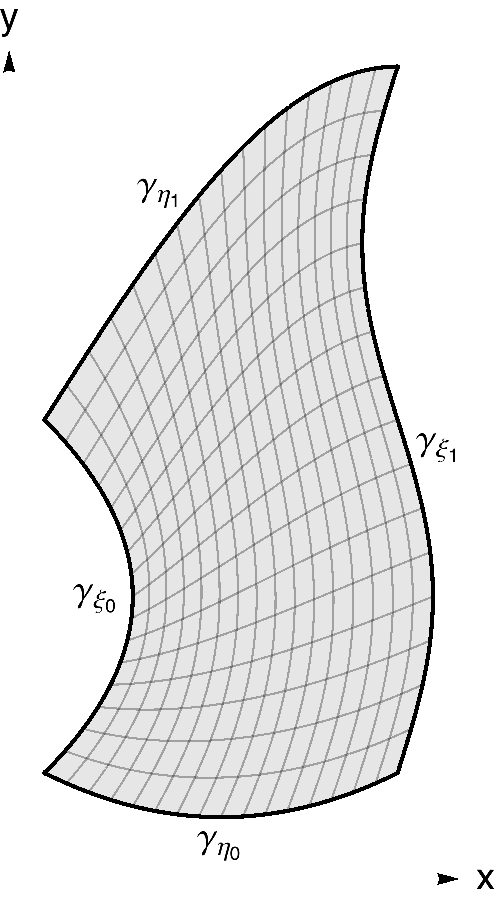
\includegraphics[width=.35\textwidth]{fig/testfig1.pdf}
\hspace{1cm}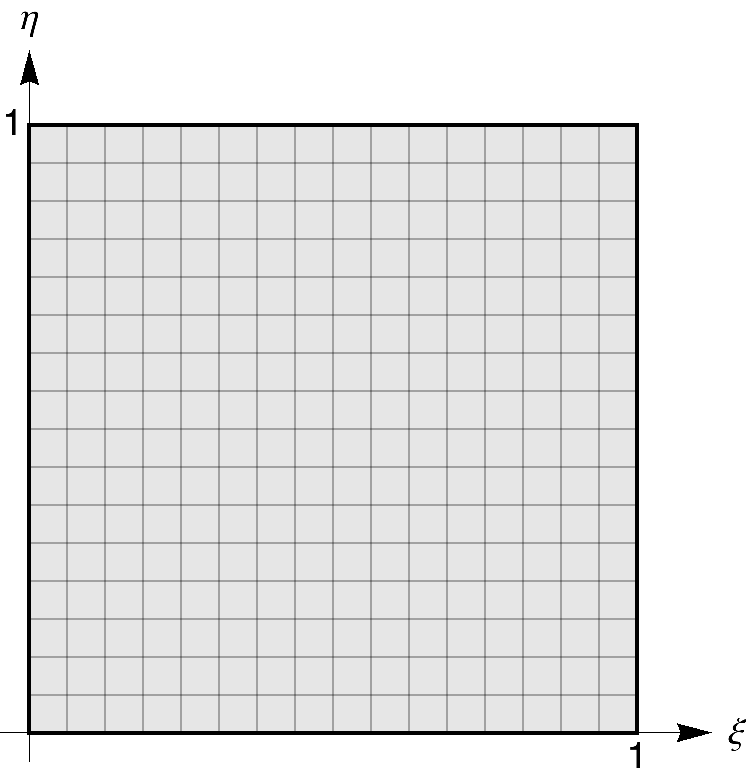
\includegraphics[width=.45\textwidth]{fig/testfig2.pdf}}
\caption{Figure Captions.}
\label{fig:label}
\end{figure}

\end{section}

\begin{section}{Analysis Methods}
\begin{subsection}{Data}
The analysis begins with data based on a sample of proton-proton collisions collected by the Compact Muon Solenoid (CMS) detector in the LHC. ``Interesting'' events are selected by the first level of the CMS trigger system which uses information from the detector's calorimeters and muon detectors to select events for analysis in a fixed time interval of less than 4 $\mu s$. These events are then further processed by a high-level trigger processor farm, which decreases the event rate from around 100 kHz to less than 1 kHz, before the data is stored. Finally, the particle-flow algorithm reconstructs and identifies all particles from the events selected by the CMS trigger system. With the data properly processed and promptly reconstructed ``online,'' further analysis can be carried out ``offline.''
\end{subsection}
\begin{subsection}{Monte Carlo}
The analysis begins with data based on a sample of proton-proton collisions collected by the Compact Muon Solenoid (CMS) detector in the LHC. ``Interesting'' events are selected by the first level of the CMS trigger system which uses information from the detector's calorimeters and muon detectors to select events for analysis in a fixed time interval of less than 4 $\mu s$. These events are then further processed by a high-level trigger processor farm, which decreases the event rate from around 100 kHz to less than 1 kHz, before the data is stored. Finally, the particle-flow algorithm reconstructs and identifies all particles from the events selected by the CMS trigger system. With the data properly processed and promptly reconstructed ``online,'' further analysis can be carried out ``offline.''
\end{subsection}
\end{section}

\begin{section}{Results}

\end{section}



%=== Appendix ============================================
\appendix

\dsp

\chapter{Appendix Title }{\label{appendix:a}}
\begin{section}{Section Title}

Appendicitis

\end{section}
\end{mainmatter}

%----- Bibliography ----------------
\ssp
\bibliographystyle{JHEP3}
\bibliography{dissertation}

\end{document} 
